% 页面设置
\documentclass[12pt, a4paper]{article} % 字号:12,纸张:A4
\usepackage[top=2.54cm, bottom=2.54cm, left=3.18cm,right=3.18cm]{geometry} % 页边距设置
% 字体设置
\usepackage[UTF8]{ctex}
\usepackage{fontspec} % 设置字体
%\setCJKmainfont{SimSun}[AutoFakeBold=true, BoldFont={SimHei}, ItalicFont={KaiTi}] % 正文字体
%\setCJKsansfont[AutoFakeBold=3]{KaiTi} % 无衬线字体
%\setCJKmonofont[AutoFakeBold=3]{SimHei} % 等宽字体
\setmainfont{Times New Roman} % 设置主字体为新罗马体
% 文本设置
\usepackage{enumerate} % 支持小标题编号
\linespread{1.5} % 行间距1.5倍
\usepackage{indentfirst}%首段缩进
\setlength{\parindent}{2em} % 首行缩进两字符
\usepackage[hidelinks]{hyperref} % 目录添加超链接
\usepackage{zhnumber} % 章节标题中文显示
\usepackage[cmyk]{xcolor} % 文字彩色显示
% 数学支持
\usepackage{amsmath} % 数学公式支持
\usepackage{amssymb} % 数学符号支持
\usepackage{bm} % 公式加粗
\usepackage{mathrsfs} % 花体字母
\usepackage{yhmath} % 更多的数学符号
% 图片设置
\usepackage{caption} % 插入图片标题
\usepackage{float} % 控制图片位置
\usepackage{subfigure} % 图片并排
\usepackage{booktabs} % 插入表格
% 表格设置
\usepackage{multirow} % 表格自动换行
\usepackage{bigstrut} % 表格间距
\usepackage{rotating} % 表格旋转
\usepackage{tabularx} % 表格宽度
\usepackage{colortbl} % 表格颜色
\usepackage{graphicx} % 表格自动宽度

\title{第五章 \ \ \ 神经网络} % 文章标题
\author{Castor Ye} % 文章作者
\date{} % 文章时间

\begin{document} % 文档从这里开始。
\maketitle % 按照预定的模板把上面那些信息排好。
\newtheorem{definition}{定义}[section]
\newtheorem{theorem}{定理}[section]
\newtheorem{example}{例}[section]
\newtheorem{solution}{题解}
\newtheorem{algorithm}{算法}
\newtheorem{axiom}{公理}
\newtheorem{property}{性质}
\newtheorem{proposition}{命题}
\newtheorem{lemma}{引理}
\newtheorem{corollary}{推论}[section]
\newtheorem{remark}{注解}
\newtheorem{condition}{条件}
\newtheorem{conclusion}{结论}
\newtheorem{assumption}{假设}
\renewcommand{\figurename}{图} % 将图片序号改为图
\renewcommand{\tablename}{表} % 将表格序号改为表
%%%%%%%%%%%%%%%%%%%%%%%%%%%%%%%%%%%%%%%%%%%%%%%%%%%%%%%%%%%%%%%%%%%%%%%
% 文章内容从此开始
\section{神经元模型}

神经网络(neural networks)中最基本的成分是神经元(neuron)模型,即上述定义中的“简单单元”。在生物神经网络中,每个神经元与其他神经元相连,当它“兴奋”时,就会向相连的神经元发送化学物质,从而改变这些神经元内的电位;如果某神经元的电位超过了一个“阈值”(threshold),那么它就会被激活,即“兴奋”起来,向其他神经元发送化学物质。

\begin{figure}[H]
    \centering
    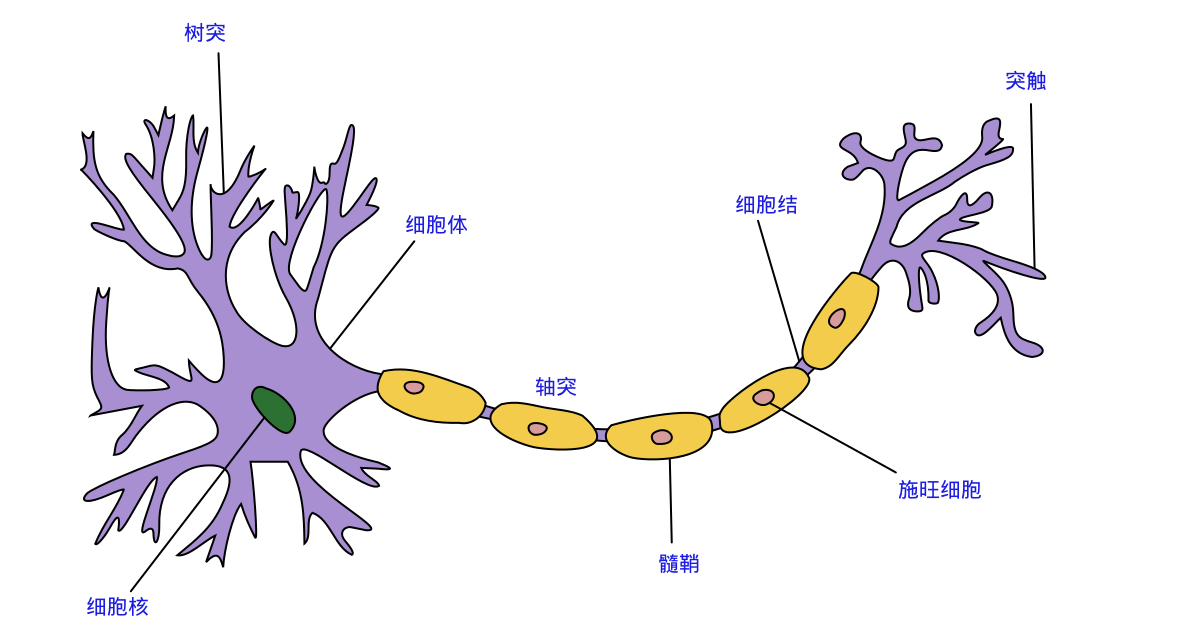
\includegraphics[width=0.8\textwidth]{../img/5-1-生物神经元.png}
    \caption{生物神经元}
    \label{fig:生物神经元}
\end{figure}

一直沿用至今的“M-P神经元模型”正是对这一结构进行了抽象,也称“阈值逻辑单元“(threshold logic unit),其中树突对应于输入部分,每个神经元收到 $n$ 个其他神经元传递过来的输入信号,这些信号通过带权重的连接传递给细胞体,这些权重又称为连接权(connection weight)。细胞体分为两部分,前一部分计算总输入值(即输入信号的加权和,或者说累积电平),后一部分先计算总输入值与该神经元阈值的差值,然后通过激活函数(activation function)的处理,产生输出从轴突传送给其它神经元。M-P 神经元模型如下图所示:

\begin{figure}[H]
    \centering
    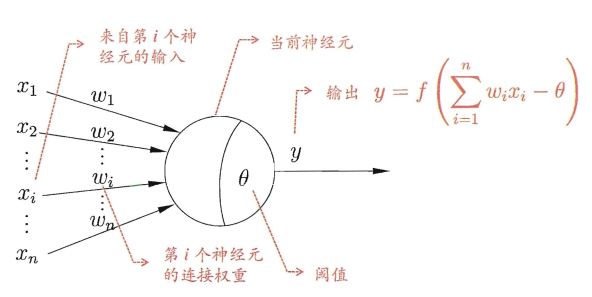
\includegraphics[width=0.8\textwidth]{../img/5-2-M-P神经元模型.png}
    \caption{M-P神经元模型}
    \label{fig:M-P神经元模型}
\end{figure}

和线性模型一样,理想中的激活函数是阶跃函数,它将输入值映射为输出值“$0$”或“$1$”。显然,“$1$”对应于神经元兴奋,“$0$”对应于神经元抑制。然而,阶跃函数具有不连续、不平滑等不太好的性质,因此实际常用 Sigmoid 函数作为激活函数。Sigmoid函数将可能在较大范围内变化的输入值挤压到 $(0, 1)$ 输出值范围内,因此也称为“挤压函数”(squashing function)。

把许多个这样的神经元按一定的层次结构连接起来,就得到了神经网络。

\section{感知机与多层网络}

感知机(Perceptron)由两层神经元组成,输入层接收外界输入信号后传递给输出层,输出层是 M-P 神经元。感知机能容易地实现逻辑与、或、非运算,注意到 $\displaystyle y = f( \sum_i w_i x_i - \theta)$,假定 $f$ 是阶跃函数,则有:

\begin{enumerate}[\hspace*{2em} i.]
    \item “与”($x_1 \wedge x_2$):令 $w1 = w2 = 1, \theta = 2$,则 $y = f(1 \cdot x_1 + 1 \cdot x_2 - 2)$,仅在 $x_1 = x_2 = 1$ 时,$y = 1$。
    \item “或”($x_1 \vee x_2$):令 $w_1 = w_2 = 1, \theta = 0.5$,则 $y = f(1 \cdot x_1 + 1 \cdot x_2 - 0.5)$,当 $x_1 - 1$ 或 $x_2 = 1$ 时,$y = 1$。
    \item “非”($\neg x_1$):令 $w_1 = -0.6, w_2 = 0, \theta = - 0.5$,则 $y = f(-0.6 \cdot x_1 + 0 \cdot x_2 + 0.5)$,当 $x_1 = 1$ 时,$y = 0$;当 $x_1 = 0$ 时,$y = 1$。
\end{enumerate}

\begin{figure}[H]
    \centering
    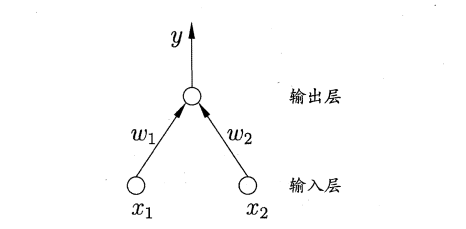
\includegraphics[width=0.5\textwidth]{../img/5-4-两个输入神经元的感知机网络结构示意图.png}
    \caption{两个输入神经元的感知机网络结构示意图}
    \label{fig:两个输入神经元的感知机网络结构示意图}
\end{figure}

更一般地,给定训练数据集,权重 $w_i(i = 1, 2, \cdots, n)$ 以及阈值 $\theta$ 可通过学习得到。阈值 $\theta$ 可看作一个固定输入为 $-1$ 的“哑结点”(dummy node)所对应的连接权重 $w_{n + 1}$,这样,权重和阈值的学习就可统一为权重的学习。感知机学习规则非常简单,对训练样例 $(x, y)$,若当前感知机的输出为 $\hat{y}$,则感知机权重将这样调整:

\begin{equation*}
    w_1 \leftarrow w_i + \Delta w_i, \ \ \ \ \Delta w_i = \eta (y - \hat{y}) x_i
\end{equation*}

其中 $\eta \in (0, 1)$ 称为学习率(learning rate)。可以看出,如果感知机对训练样例 $(x, y)$ 预测正确而,即 $\hat{y} = y$,则感知机不发生变化,否则将根据错误的程度进行权重调整。

由于感知机模型只有一层功能神经元,因此其功能十分有限,只能处理线性可分的问题,对于这类问题,感知机的学习过程一定会收敛(converge),因此总是可以求出适当的权值。但是对于像书上提到的异或问题,只通过一层功能神经元往往不能解决,因此要解决非线性可分问题,需要考虑使用多层功能神经元,即神经网络。

\begin{figure}[H]
    \centering
    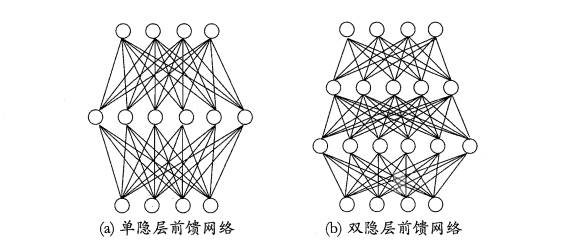
\includegraphics[width=0.8\textwidth]{../img/5-5-多层前馈神经网络结构示意图.png}
    \caption{多层前馈神经网络结构示意图}
    \label{fig:多层前馈神经网络结构示意图}
\end{figure}

在神经网络中,输入层与输出层之间的层称为隐含层或隐层(hidden layer),隐层和输出层的神经元都是具有激活函数的功能神经元。只需包含一个隐层便可以称为多层神经网络,常用的神经网络称为“多层前馈神经网络”(multi-layer feedforward neural network),该结构满足以下几个特点:

\begin{enumerate}[\hspace*{2em} i.]
    \item 每层神经元与下一层神经元之间完全互连。
    \item 神经元之间不存在同层连接。
    \item 神经元之间不存在跨层连接。
\end{enumerate}

根据上面的特点可以得知:这里的“前馈”指的是网络拓扑结构中不存在环或回路,而不是指该网络只能向前传播而不能向后传播(下节中的BP神经网络正是基于前馈神经网络而增加了反馈调节机制)。神经网络的学习过程就是根据训练数据来调整神经元之间的“连接权”以及每个神经元的阈值,换句话说:神经网络所学习到的东西都蕴含在网络的连接权与阈值中。

\section{误差逆传播算法(BP 神经网络)}

由上面可以得知:神经网络的学习主要蕴含在权重和阈值中,多层网络的学习能力比单层感知机強得多,简单感知机学习规则显然已经不够用了。误差逆传播(error BackPropagation, BP)算法正是为学习多层前馈神经网络设计,其是迄今为止最为成功的神经网络学习算法。

给定训练集 $D = \{(x_1, y_1), (x_2, y_2), \cdots, (x_m, y_m)\}, x_i \in \mathbb{R}^d, y_i \in \mathbb{R}^l$,即输入示例由 $d$ 个属性描述,输出 $l$ 维实值向量。

为便于讨论,下图给出了一个拥有 $d$ 个输入神经元、$l$ 个输出神经元、$q$ 个隐层神经元的多层前馈神经网络结构,其中输出层第 $j$ 个神经元的阈值用 $\theta_j$ 表示,隐层第 $h$ 个神经元的阈值用 $\gamma_h$ 表示。输入层第 $i$ 个神经元与隐层第 $h$ 个神经元之间的连接权为 $v_{ih}$,隐层第 $h$ 个神经元与输出层第 $j$ 个神经元之间的连接权为 $w_{hj}$。

记隐层第 $h$ 个神经元接收到的输入为 $\displaystyle \alpha_h = \sum_{i = 1}^{d} v_{ih} x_i$,输出层第 $j$ 个神经元接收到的输入为 $\displaystyle \beta_{j} = \sum_{h = 1}^{q} w_{hj}b_h$,其中 $b_h$ 为隐层第 $h$ 个神经元的输出。

\begin{figure}[H]
    \centering
    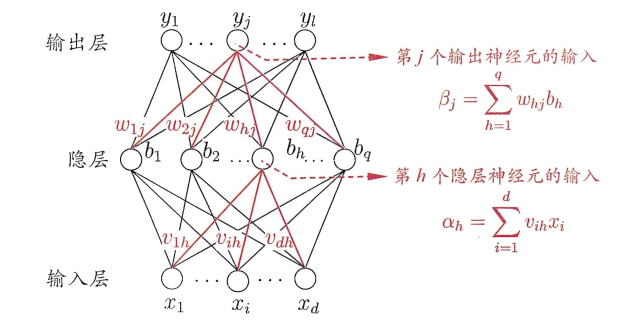
\includegraphics[width=0.8\textwidth]{../img/5-6-BP网络及算法中的变量符号.png}
    \caption{BP网络及算法中的变量符号}
    \label{fig:BP网络及算法中的变量符号}
\end{figure}

对训练例 $(x_k, y_k)$,假定神经网络的输出为 $\hat{y}_k = (\hat{y}_1^k, \hat{y}_2^k, \cdots, \hat{y}_l^k)$,即:
\begin{equation*}
    \hat{y}_j^k = f(\beta_j - \theta_j)
\end{equation*}
则网络在 $(x_k, y_k)$ 上的均方差为:
\begin{equation*}
    E_k = \frac{1}{2} \sum_{j = 1}^{l} (\hat{y}_j^k - y_j^k)^2
\end{equation*}

图 \ref{fig:BP网络及算法中的变量符号} 的网络中有 $(d + l + 1) q + l$ 个参数需确定:
\begin{enumerate}[\hspace*{2em} i.]
    \item 输入层到隐层的 $d \cdot q$ 个权值。
    \item 隐层到输出层的 $q \cdot l$ 个权值。
    \item $q$ 个隐层神经元的阈值。
    \item $l$ 个输出层神经元的阈值。
\end{enumerate}

$BP$ 是一个迭代学习算法,在迭代的每一轮中采用广义的感知机学习规则对参数进行更新估计,任意参数 $v$ 的更新估计式为:
\begin{equation*}
    v \leftarrow v + \Delta v
\end{equation*}
下面以图 \ref{fig:BP网络及算法中的变量符号} 中隐层到输出层的连接权 $w_{hj}$ 为例来进行推导。

$BP$ 算法基于梯度下降(gradient descent)策略,以目标的负梯度方向对参数进行调整,给定学习率 $\eta$,有:
\begin{equation*}
    \Delta w_{hj} = - \eta \frac{\partial E_k}{\partial w_{hj}}
\end{equation*}
注意到 $w_{hj}$ 先影响到第 $j$ 个输出层神经元的输入值 $\beta_{j}$,再影响到其输出值 $\hat{y}_j^k$,然后影响到 $E_k$,有:
\begin{equation*}
    \frac{\partial E_k}{\partial w_{hj}} = \frac{\partial E_k}{\partial \hat{y}_j^k} \cdot \frac{\partial \hat{y}_j^k}{\partial \beta_{j}} \cdot \frac{\partial \beta_j}{\partial w_{hj}}
\end{equation*}

根据 $\beta_{j}$ 的定义,显然有:
\begin{equation*}
    \frac{\partial \beta{j}}{\partial w_{hj}} = b_h
\end{equation*}

同时,Sigmoid 函数有一个很好的性质:
\begin{equation*}
    f^{\prime} (x) = f(x) (1 - f(x))
\end{equation*}

根据前式则有:
\begin{equation*}
    \begin{array}{*{20}{l}}
        {g_j}&{\displaystyle = - \frac{\partial E_k}{\partial \hat{y}_j^k} \cdot \frac{\partial \hat{y}_j^k}{\partial \beta_j} }\\
        {}&{ = - (\hat{y}_j^k - y_j^k) f^{\prime} (\beta_j - \theta_j) } \\
        {}&{= \hat{y}_j^k (1 - \hat{y}_j^k) (y_j^k - \hat{y}_j^k)}
    \end{array}
\end{equation*}

代入前式得到 $BP$ 算法中关于 $w_{hj}$ 的更新公式:
\begin{equation*}
    \Delta w_{hj} = \eta g_j b_h
\end{equation*}
类似可得:
\begin{equation*}
    \Delta \theta_{j} = - \eta g_j, \ \ \ \Delta v_{ih} = \eta e_h x_i, \ \ \ \Delta \gamma_h = - \eta e_h
\end{equation*}
则有:
\begin{equation*}
    \begin{array}{*{20}{l}}
        {e_h}&{\displaystyle  = - \frac{\partial E_k}{\partial b_h} \cdot \frac{\partial b_h}{\partial \alpha_h} }\\
        {}&{\displaystyle  = - \sum_{j = 1}^{l} \frac{\partial E_k}{\partial \beta_j} \cdot \frac{\partial \beta_j}{\partial b_h} f^{\prime} (\alpha_h - \gamma_h)} \\
        {}&{\displaystyle  = \sum_{j = 1}^{l} w_{hj} g_{j} f^{\prime} (\alpha_h - \gamma_h) } \\
        {}&{\displaystyle  = b_h (1 - b_h) \sum_{j = 1}^{l} w_{hj} g_{j} }
    \end{array}
\end{equation*}

学习率 $\eta \in (0, 1)$ 控制这算法每一轮迭代中的更新步长,若太大则容易振荡,太小则收敛速度又会过慢。

下图给出了 $BP$ 算法的工作流程。对每个训练样例,$BP$ 算法执行以下操作:先将输入示例提供给输入层神经元,然后逐层将信号前传,知道产生输出层的结果;然后计算输出层的误差,再将误差逆向传播至隐层神经元,最后根据隐层神经元的误差来对连接权和阈值进行调整。

\begin{figure}[H]
    \centering
    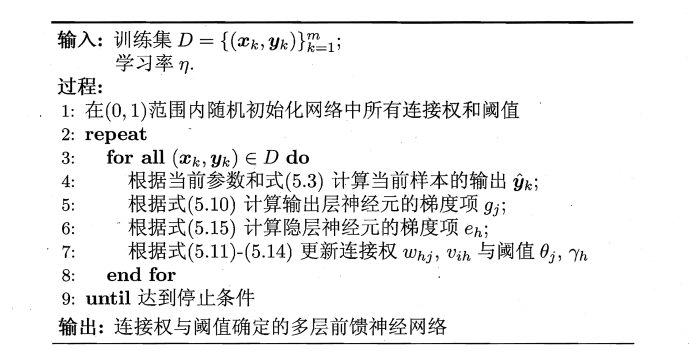
\includegraphics[width=0.8\textwidth]{../img/5-7-误差逆传播算法.png}
    \caption{误差逆传播算法}
    \label{fig:误差逆传播算法}
\end{figure}

需注意的是,$BP$ 算法的目标是要最小化训练集 $D$ 上的积累误差:
\begin{equation*}
    E = \frac{1}{m} \sum_{k = 1}^{m} E_k
\end{equation*}

如果基于累积误差最小化的更新规则,则得到了累积误差逆传播算法(accumulated error backpropagation),即每次读取全部的数据集一遍,进行一轮学习,从而基于当前的累积误差进行权值调整,因此参数更新的频率相比标准BP算法低了很多,但在很多任务中,尤其是在数据量很大的时候,往往标准BP算法会获得较好的结果。另外对于如何设置隐层神经元个数的问题,至今仍然没有好的解决方案,常使用“试错法”进行调整。

前面提到,BP神经网络强大的学习能力常常容易造成过拟合问题,有以下两种策略来缓解BP网络的过拟合问题:

\begin{enumerate}[\hspace*{2em} i.]
    \item 早停:将数据分为训练集与测试集,训练集用于学习,测试集用于评估性能,若在训练过程中,训练集的累积误差降低,而测试集的累积误差升高,则停止训练。
    \item 引入正则化(regularization):基本思想是在累积误差函数中增加一个用于描述网络复杂度的部分,例如所有权值与阈值的平方和,其中λ∈(0,1)用于对累积经验误差与网络复杂度这两项进行折中,常通过交叉验证法来估计。
    \begin{equation*}
        E = \lambda \frac{1}{m} \sum_{k = 1}{m} E_k + (1 - \lambda) \sum_{i} w_i^2
    \end{equation*}
\end{enumerate}

\section{全局最小与局部极小}

模型学习的过程实质上就是一个寻找最优参数的过程,例如BP算法试图通过最速下降来寻找使得累积经验误差最小的权值与阈值,在谈到最优时,一般会提到局部极小(local minimum)和全局最小(global minimum)。

\begin{enumerate}[\hspace*{2em} i.]
    \item 局部极小解:参数空间中的某个点,其邻域点的误差函数值均不小于该点的误差函数值。
    \item 全局最小解:参数空间中的某个点,所有其他点的误差函数值均不小于该点的误差函数值。
\end{enumerate}

\begin{figure}[H]
    \centering
    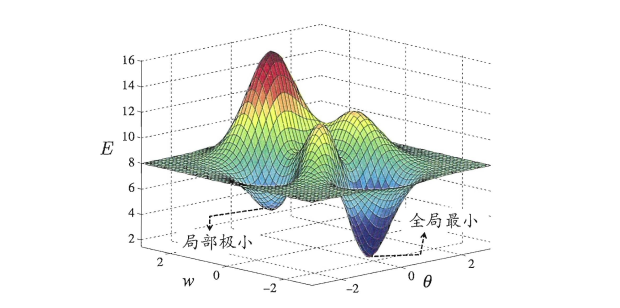
\includegraphics[width=0.8\textwidth]{../img/5-8-全局最小与局部最小.png}
    \caption{全局最小与局部最小}
    \label{fig:全局最小与局部最小}
\end{figure}

要成为局部极小点,只要满足该点在参数空间中的梯度为零。局部极小可以有多个,而全局最小只有一个。全局最小一定是局部极小,但局部最小却不一定是全局最小。显然在很多机器学习算法中,都试图找到目标函数的全局最小。梯度下降法的主要思想就是沿着负梯度方向去搜索最优解,负梯度方向是函数值下降最快的方向,若迭代到某处的梯度为0,则表示达到一个局部最小,参数更新停止。因此在现实任务中,通常使用以下策略尽可能地去接近全局最小。

\begin{enumerate}[\hspace*{2em} i.]
    \item 以多组不同参数值初始化多个神经网络,按标准方法训练,迭代停止后,取其中误差最小的解作为最终参数。
    \item 使用“模拟退火”技术,这里不做具体介绍。
    \item 使用随机梯度下降,即在计算梯度时加入了随机因素,使得在局部最小时,计算的梯度仍可能不为0,从而迭代可以继续进行。
\end{enumerate}

\section{深度学习}

理论上,参数越多,模型复杂度就越高,容量(capability)就越大,从而能完成更复杂的学习任务。深度学习(deep learning)正是一种极其复杂而强大的模型。

怎么增大模型复杂度呢?两个办法,一是增加隐层的数目,二是增加隐层神经元的数目。前者更有效一些,因为它不仅增加了功能神经元的数量,还增加了激活函数嵌套的层数。但是对于多隐层神经网络,经典算法如标准BP算法往往会在误差逆传播时发散(diverge),无法收敛达到稳定状态。

那要怎么有效地训练多隐层神经网络呢?一般来说有以下两种方法:

\begin{enumerate}[\hspace*{2em} i.]
    \item 无监督逐层训练(unsupervised layer-wise training):每次训练一层隐节点,把上一层隐节点的输出当作输入来训练,本层隐结点训练好后,输出再作为下一层的输入来训练,这称为预训练(pre-training)。全部预训练完成后,再对整个网络进行微调(fine-tuning)训练。一个典型例子就是深度信念网络(deep belief network,简称DBN)。这种做法其实可以视为把大量的参数进行分组,先找出每组较好的设置,再基于这些局部最优的结果来训练全局最优。
    \item 权共享(weight sharing):令同一层神经元使用完全相同的连接权,典型的例子是卷积神经网络(Convolutional Neural Network,简称CNN)。这样做可以大大减少需要训练的参数数目。
\end{enumerate}

\begin{figure}[H]
    \centering
    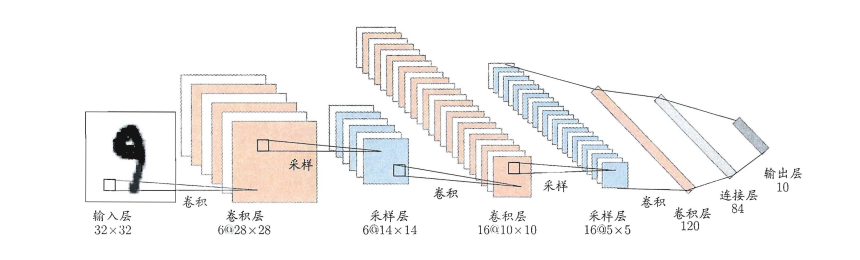
\includegraphics[width=0.8\textwidth]{../img/5-9-卷积神经网络用于手写数字识别.png}
    \caption{卷积神经网络用于手写数字识别}
    \label{fig:卷积神经网络用于手写数字识别}
\end{figure}

深度学习可以理解为一种特征学习(feature learning)或者表示学习(representation learning),无论是DBN还是CNN,都是通过多个隐层来把与输出目标联系不大的初始输入转化为与输出目标更加密切的表示,使原来只通过单层映射难以完成的任务变为可能。即通过多层处理,逐渐将初始的“低层”特征表示转化为“高层”特征表示,从而使得最后可以用简单的模型来完成复杂的学习任务。

传统任务中,样本的特征需要人类专家来设计,这称为特征工程(feature engineering)。特征好坏对泛化性能有至关重要的影响。而深度学习为全自动数据分析带来了可能,可以自动产生更好的特征。

\end{document}